\header{
    \headtitle{Gaudeamus Igitur} \label{gaudeamus-igitur}
    %
    \insertComment{Chant international des étudiants qui daterait du 13ème siècle. Il est considéré comme le plus ancien chant estudiantin et comme l'incarnation de la vie libre et facile de l'étudiant.}{Réécrit au milieu du 18ème siècle, il est chanté à travers le monde entier.}
}

\enluminure{4}{\href{https://www.youtube.com/watch?v=aLUKfU2AOBY}{G}}\\ 
$\left.\begin{tabular}{l}
\hspace{-0.4cm}
\textsc{audeamus} igitur,             ~~~~~~~~~
\\
\hspace{-0.4cm}
Juvenes dum sumus                   ~~~~~~~~~~~~
\end{tabular}\right\rbrace$ bis
\\Post Jucundam juventutem,
\\Post molestam senectutem 
\\Nos habebit humus     \bissimple
\dualcol{
    \bisdouble{Ubi sunt, qui ante nos ~~~}
    {In mundo fuere ? }
    Vadite ad superos, 
    \\Transite ad inferos, 
    \\Ubi iam fuere            ~~~~~~~~~~~~~~~~\bissimple
    \\
    \bisdouble{Vita nostra brevis est,  ~~~}
    {Brevi finietur;}
    Venit mors velociter, 
    \\Rapit nos atrociter; 
    \\Nemini parcetur            ~~~~~~~~~~~~~\bissimple
    \\
    \bisdouble{Vivat academia            ~~~~  ~~~}
    {Vivant professores,            ~~~~  ~~~}
    Vivat membrum quod libet, 
    \\Vivant membra quae libet; 
    \\Semper sint in flore            ~~~~~~~~~\bissimple
    \\
    \bisdouble{Vivant omnes virgines, ~~}
    {Faciles, formosae, }
    Vivant et mulieres, 
    \\Tenerae, amabiles,
    \\Bonae, laboriosae            ~~~~~~~~~~~\bissimple
    \\
    \bisdouble{Vivat et respublica   ~~~~~~~}
    {Et qui illam regit,    ~~~~~~~}
    Vivat nostra civitas, 
    \\Maecenatum caritas, 
    \\Quae nos hic protegit      ~~~~~~\bissimple
    \\
    \bisdouble{Pereat tristitia,              ~~~~~~~~~~~~}
    {Pereant osores,              ~~~~~~~~~}
    Pereat diabolus 
    \\Quivis antiburschius, 
    \\Atque irrisores             ~~~~~~~~~~~~~~~\bissimple
}

\begin{center}
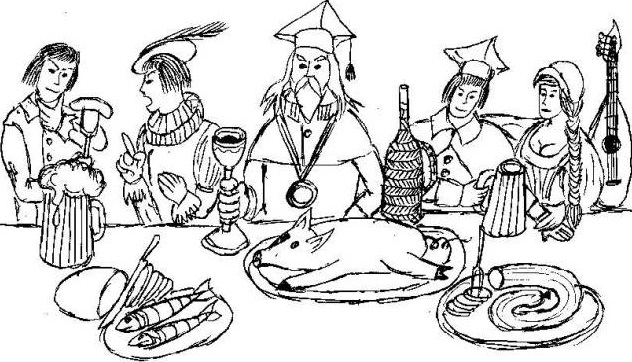
\includegraphics[width=0.5\textwidth]{images/Gaudeamus.JPG}
\end{center}

\breakpage